%%%%%%%%%%%%%%%%%%%%%%%%%%%%%%%%%%%
%                 Wrocław, grudzień 2012r.
%    Pracownia z Analizy Numerycznej M
%      Sprawozdanie z zadania p2.2
%         Łukasz Czapliński
%%%%%%%%%%%%%%%%%%%%%%%%%%%%%%%%%%%
\documentclass[11pt,wide]{mwart}

\usepackage[utf8]{inputenc} 
\usepackage[OT4,plmath]{polski}
\usepackage{graphicx}      
\usepackage{caption}
\usepackage{subcaption}
\usepackage{longtable}
\usepackage{amsmath,amssymb,amsfonts,amsthm,mathtools}

\usepackage{bbm}           
\usepackage[colorlinks=true]{hyperref}
                          
\usepackage{url}
%%%%%%%%%%%%%%%%%%%%%%%%%%%%%%%%%5
\title{{\textbf{Pracownia z analizy numerycznej\\}}
       {\Large Sprawozdanie do zadania \textbf{P3.7}\\}
       {\large Prowadzący: dr Paweł Woźny}}
\author{Łukasz Czapliński\\  e-mail: \texttt{czapl.luk@gmail.com}}
\date{Wrocław, dnia \today\ r.}

\begin{document}
\thispagestyle{empty}
\maketitle
\newpage
\section{Wstęp}
\subsection{Słowo wstępu}
Do jednego z najczęściej spotykanych i jednocześnie często najtrudniejszym do rozwiązania problemów matematycznych należy zagadnienie liczenia całek oznacznonych. Często rozwiązanie równania wymaga policzenia takich całek, a jeśli tylko całka nieoznaczona z danej funkcji pozwala się wyrazić w prosty sposóp, to problem się nagle staje bardzo złożony i trudny do ominięcia. Jednym z prostszych pomysłow na rozwiązanie tego problemu jest liczenie całki nie z danej funkcji, lecz z innej, prostszej. Użycie tutaj zwykłej interpolacji wielomianowej daje niezadowalające wyniki (przynajmniej na pierwszy rzut oka, ponieważ prowadzi do kwadratury Newtona-Cotesa, która jak wiadomo nie zawsze jest zbieżna). Rozważmy zatem inny sposób interpolacji - naturalna funkcję sklejaną 3-ciego stopnia. Wiadomo, że jest ona "najgładsza" z funkcji interpolujących, więc błąd nie powinien być duży. W tej pracowni sprawdzę, jak to działa w praktyce.
\subsection{Oznaczenia i wzory}
\begin{table}[!h]
  \centering
  \begin{tabular}{r | l}
    \hline
    Symbol & Znaczenie \\
    \hline
    NFSI3 & Naturalna funkcja sklejana interpolujaca 3-ciego stopnia \\
    $s(x)$ & NFSI3 \\
    $M_k$ & Momenty we wzorze na $s(x)$: $M_k=s"(x_k), k=0,1,..n$\\
    \hline
  \end{tabular}
  \caption{Uzyte oznaczenia}
\end{table}
Wzór na błąd przybliżenia funkcji $f$  przez NFSI3: $s$ jest dany następującym wzorem:\\
\begin{center}
  $\lVert{s-f}\rVert_{\infty,[x_0,x_n]}\sim\frac{5}{384}$ $\dot\lVert{f^{(4)}}\rVert_{\infty,[x_0,x_n]}\dot h^4$
  \label{WZOR}
\end{center}
Możnaby z tego wnioskować, że dobór punktów kluczowych nie powinien mieć dużego znaczenia, o ile nie będą tylko zbyt skupione w jednym miejscu. Postanowiłem to też sprawdzić i wykonywałem testy dla dwóch metod: jednej z równoodległymi punktami kluczowymi i drugiej z lekko zaburzonymi tak, by odległość między nimi była równa co najwyżej $3*h$.
\subsection{Opis metod}
Do znalezienia naturalnej funkcji sklejanej 3-ciego stopnia poniższego następującego algorytmu (\ref{algorytm}), którego poprawność została omówiona i udowodniona na ćwiczeniach z analizy numerycznej (II UWr 2012/2013, nie jest to jednak trudne).
\begin{table}[!h]
  \centering
  \begin{tabular}{|p{0.8\linewidth}|}
    \hline
    Wiadomo, że $M_k$ spełniają układ równań:\\
    $
    \lambda_kM_{k-1} + 2M_k + (1-\lambda_k)M_{k+1} = d_k
    $, gdzie\\
    $d_k:=6f[x_{k-1},x_k,x_{k+1}]$, $\lambda_k:=h_k/(h_k+h_{k+1})$,$h_k:=x_k- x_{k-1}$.\\
    Układ ten tworzy prostą do rozwiązania macierz, w której pierwszy i ostatni wiersz zawierają po 2 niezerowe wyrazy, a wszystkie pozostałe po 3, podobnie kolumny. Można go rozwiązać w następujący sposób:\\\\
    \hline
    Obliczamy pomocnicze wartości $p_1,p_2,...,p_{n-1}, q_0,q_1,...,q_{n-1}, u_0,u_1,...,u_{n-1}$\\ w natępujący rekurencyjny sposób:\\
    $q_0:=u_0:=0$,\\
    \begin{math}
      \left\{ 
      \begin{array}{l}
        p_k:=\lambda_kq_{k-1}+2 \\
        q_k:=(\lambda_k-1)/p_k \\
        u_k:=(d_k-\lambda_ku_{k-1})/p_k
      \end{array} 
    \right\} (k=1,2,...,n-1)
    \end{math}
    \\Wówczas:\\
    $M_{n-1}=u_{n-1},$\\$M_k=u_k+q_kM_{k+1} (k=n-2,n-3,...,1)$
    \\\hline
  \end{tabular}
  \caption{Algorytm obliczania współczynników NFSI3}
  \label{algorytm}
\end{table}
\\\indent
Jak widać, koszt realizacji algorytmu jest liniowo zależny od ilości węzłów. Z kolei do obliczania wartości funkcji i całki użyto jawnego wzoru na NFSI3 w każdym z podprzedziałów, więc koszt liczenia całki jest zależny od ilości podprzedziałów, w których trzeba wartość całki nieoznaczonej z NFSI3 obliczyć. Można byłoby zamiast tego poprzekształcać wzór na całkę, aby uzyskać mniej działań artymetycznych, a zatem również mniejszy błąd, jednak zysk nie byłby znaczący. 
Zatem koszt obliczeń jest podobny do tego, jaki niesie ze sobą kwadratura Newtona-Cotesa (zwykła, jak i złożona). Jak w porównaniu z nimi plasuje się omawiana metoda?
\subsection{O programie}
Aby rzetelnie odpowiedzieć na to pytanie, napisany został obszerny program testujący. Składa się on z kilku modułów.
Pierwszy z nich odpowiada za parsowanie i obliczanie wartości funkcji. 
Znajduje się w pliku fhb.cpp.
Pozwala na stworzenie struktury \begin{verbatim}fhb::fun_wrap\end{verbatim} za pomocą konstruktora \begin{verbatim}fhb::fun_wrap(string s)\end{verbatim} gdzie s zawiera wzór funkcji - więcej o nim dalej - i liczenie wartości tej funkcji w punkcie x za pomocą metody \begin{verbatim}double fhb::fun_wrap::apply(double x)\end{verbatim}
Kolejny, zawarty już w program.cpp odpowiada za implementację omawianej metody.
NFSI3 jest reprezentowana przez tablicę par: $[(x_k,M_k)] (k=0,1,...n)$. Funkcja 
\begin{verbatim}
spline_params(fhb::fun_wrap, vector<double>)
\end{verbatim} 
oblicza owe wartości dla danej funkcji i tablicy punktów kluczowych: $[x_k]$. Funkcja 
\begin{verbatim}
double spline_at(fhb::fun_wrap, pair<double, double>, pair<double, double>, double)
\end{verbatim} 
zwraca wartość NFSI3 w danym punkcie $x$, zakładając że mieści się on w przedziale którego parametry ta funkcja ta otrzymuje. Podobnie funkcja 
\begin{verbatim}
double spline_int_at(fhb::fun_wrap, pair<double, double>, pair<double, double>, double)
\end{verbatim}
, z tym że ta zwraca wartość całki w danym $x$. Większą część pracy wykonują funkcje 
\begin{verbatim}
double integral_approx_at_points(fhb::fun_wrap, vector<double>, double)
\end{verbatim} 
oraz 
\begin{verbatim}
void integral_lim_n(fhb::fun_wrap, double, double, double)
\end{verbatim}
. Pierwsza z nich zwraca wartość przybliżenia całki oznaczonej przez naszą metodę dla danej funkcji, tablicy punktów kluczowych i $x$-a. Druga korzysta z niej by stworzyć listy tych przybliżen dla liczby punktów kluczowych $n=0,1,..100$z punktami równoodległymi i lekko zaburzonymi (tak, by maksymalna odległość między punktami była maksymalnie 3x większa niż poprzednio).
\\Trzeci moduł to funkcja 
\begin{verbatim}
void do_computations(string, string)
\end{verbatim} 
która odpowiada za komunikację programu z użytkownikiem.
Przyjmuje jako argument nazwę metody (tutaj po prostu Integrals, bez znaczenia) i testu, który ma być wykonany, następnie wczytuje test z pliku \begin{verbatim}"./testy/<nazwa_testu>.din"\end{verbatim} i wypisuje kolejno wyniki:\\
\begin{tabular}{l l}
   \hline
  co?                                                       & gdzie? - nazwa pliku\\
  \hline
  ciąg zgodnych miejsc dziesiętnych dla obu metod           & 
    \begin{minipage}{3in} \begin{verbatim}"./wyniki/<nazwa_testu>/<nazwa_metody>.dd"\end{verbatim} 
      \end{minipage}\\
  statystyki (czas, ilość iteracji, średni rząd zbieżności) & 
    \begin{minipage}{3in} \begin{verbatim}"./wyniki/statistics.tex"\end{verbatim} 
      \end{minipage}\\
\end{tabular}
\indent Ogólnie sam program przyjmuje jako argument nazwę testu i wywołuje 
\begin{verbatim}do_computations\end{verbatim} dla wszystkich niego.
Dodatkowo zamieszczone zostały skrypty (w folderze "./skrypty"). Główny z nich - replot.sh - upewnia się, że istnieje odpowiednia struktura katalogów (tworzy wymagane, jeśli ich nie ma), kompiluje program, wywołuje go dla każdego testu z foldery "./testy", następnie tworzy plik z poleceniem dla gnuplota, wywołuje gnuplota by stworzył wykresy i umieszcza je w folderze "./wykresy". Następnie wywołuje pdftex'a, by ponownie stworzył sprawozdanie (ze zmienionymi wykresami) i usuwa zbędne pliki.
\subsubsection{O parserze}
Używany parser z pliku
\begin{verbatim}fhb.cpp\end{verbatim}
został napisany przez autora jako projekt na ANSI C zanim poznał on słowo "parser", więc naturalnie ma pewne ograniczenia:
\begin{enumerate}
\item
  Nie obsługuje on potęg. Tak więc $x^2$ należy podać jako $x*x$.
\item
  W funkcji może występować tylko jedna zmienna i należy ją oznaczyć jako $x$.
\item
  Niedozwolone są znaki białe - nie powinna wystąpić żadna spacja we wzorze funkcji.
\item
  Obsługiwane są tylko wbudowane funkcje: $sin$, $cos$, $sqrt$, $ln$ i specjalna $mpi$. Każda z nich musi otrzymać jakiś argument - funkcję w nawiasach $( )$ lub samo $x$. Funkcja $mpi$ zwraca zawsze PI, niezależnie od argumentu.
\item
  Poza tym argument - string może być dowolną (matematycznie poprawną) funkcją składającą się ze znaków: $x$, $*$, $/$, $+$, $-$, nawiasów $( )$ i stałych.
\end{enumerate}

\subsubsection{Struktura testu}
Test powinien się składać z 4 linii. Powinny one wyglądać następująco:
\begin{enumerate}
  \item
    ciąg znaków - funkcja, której całki szukamy. Format taki, jak dla parsera.
  \item
    ciąg znaków - całka nieoznaczona powyższej funkcji. Format jw.
  \item
    ciąg znaków - 3 liczby typu double (w notacji angielskiej, $.$ zamiast $,$) - początek i koniec przedziału w którym chcemy liczyć całkę oznaczoną oraz koniec $x$ - całka będzie policzona od początku przedziału do $x$. Oddzielone dowolnym białym znakiem.
\end{enumerate}
\section{Wyniki doświadczenia}
\subsection{Ogólne spojrzenie na wyniki}
Oto pełne wyniki przeprowadzonych doświadczeń.
\begin{table}[h]
  \begin{tabular}{| l | l l l | l l l | l l|}
  \hline
  Funkcja & a & b & x & \multicolumn{3}{|c}{Wyniki} & \multicolumn{2}{|c|}{Blad }\\
  & & & & true & mono & dist & mono & dist \\
  \hline 
sin(x) & 0 & 6 & 4 & 1.65364 & 1.6524 & 1.65156 & 3.12227 & 2.90059\\
x*x*x*x-2*x-10 & -5 & 6 & 2 & 582.4 & 583.35 & 584.212 & 2.78753 & 2.50713\\
1/(x*x) & 1 & 14 & 4 & 0.75 & 0.754318 & 0.75664 & 2.23975 & 2.05288\\
sin(x)*sin(4*x)+2 & -2 & 3 & 3 & 10.0115 & 10.0118 & 10.0098 & 4.50875 & 3.77205\\
cos(6*x+6) & 41 & 81 & 45 & -0.17785 & -0.455832 & -0.698672 & -0.193965 & -0.466636\\
sin(x)+cos(x) & -1 & 2 & 1.5 & 2.30853 & 2.30774 & 2.30729 & 3.46504 & 3.26966\\
x*x*x+3 & 3 & 6 & 5.5 & 216.016 & 216.037 & 216.047 & 3.99609 & 3.84353\\
sin(x)*2 & 5 & 7 & 5.5 & -0.850015 & -0.849822 & -0.849758 & 3.64289 & 3.51847\\
    \hline  
  \end{tabular}\\\\
  \begin{tabular}{r | l}
  Oznaczenie & znaczenie \\
  \hline
  Funkcja & całkę z niej przybliżaliśmy \\
  a & początek przedziału \\
  b & koniec przedziału  na którym przybliżaliśmy funkcję przez NFSI3\\
  x & koniec przedziału całkowania \\
  Wyniki: & \\
  true & prawdziwa wartość \\
  mono & dla punktów kluczowych równoodległych \\
  dist & dla zaburzonych punktów kluczowych \\
  Błąd & \\
  mono & jw. \\
  dist & jw.
  \end{tabular}
\end{table}

Jak widać, dla większości testów $n=100$ dawało około 3 miejsc zerowych dokładności, przy czym wyniki dla bardziej oddalonych od siebie punktów kluczowych były niewiele gorsze od tych dla równoodległych (zgadza się to ze wzorem na błąd przybliżenia przez NFSI3). Cóż wobec tego można powiedzieć o ogólnej zbieżności metod? Spójrzmy na wykresy dla testu 0 i 3 (\ref{fig:test0} i \ref{fig:test3}).\\
\begin{figure}[!h]
  \begin{minipage}[b]{0.45\linewidth}
    \centering
    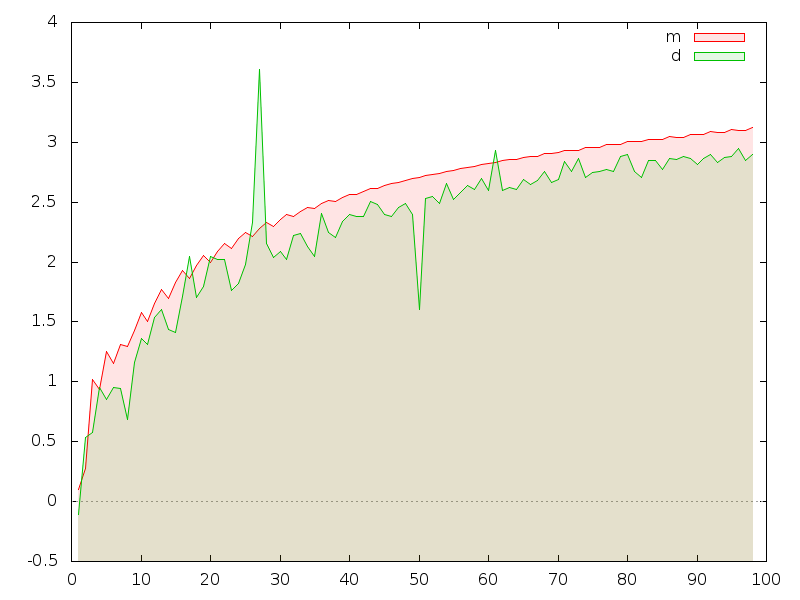
\includegraphics[width=\linewidth]{../wykresy/test0_diff.png}
    \caption{Wykres błędu dla testu 0}
    \label{fig:test0}
  \end{minipage}
  \hspace{0.5cm}
  \begin{minipage}[b]{0.45\linewidth}
    \centering
    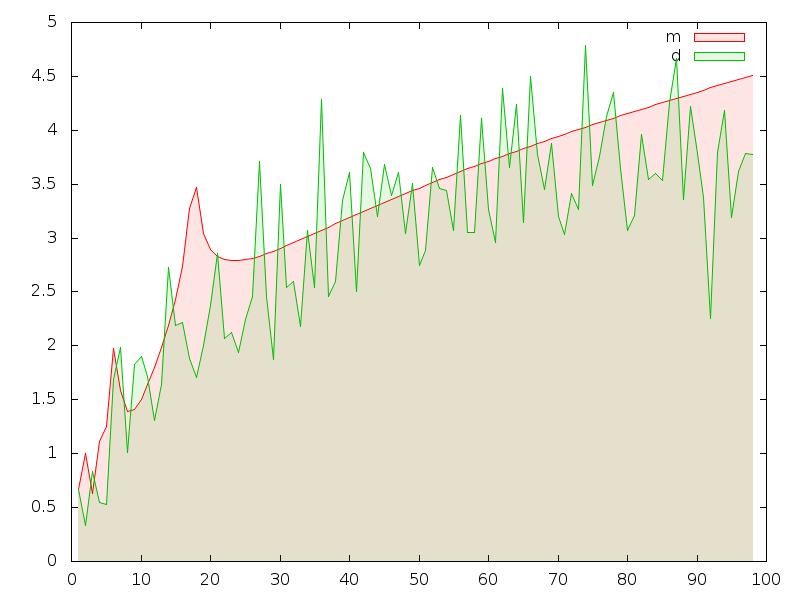
\includegraphics[width=\linewidth]{../wykresy/test3_diff.png}
    \caption{Wykres błedu dla testu 3}
    \label{fig:test3}
  \end{minipage}
\end{figure}
Z wykresów wynika, że przynajmniej dla $n\in{0,1,...100}$ metoda jest zbieżna zarówno dla równoodległych punktów, jak i zaburzonych. Jednak ilość zgodnych cyfr dziesiętnych rośnie jak $\log{n}$, a więc niezbyt szybko. Z tabeli wynika też że dla jednego testu błąd był bardzo duży. Spójrzmy na wykresy \ref{fig:test41} i \ref{fig:test42}.\\
\begin{figure}[!h]
  \begin{minipage}[b]{0.45\linewidth}
    \centering
    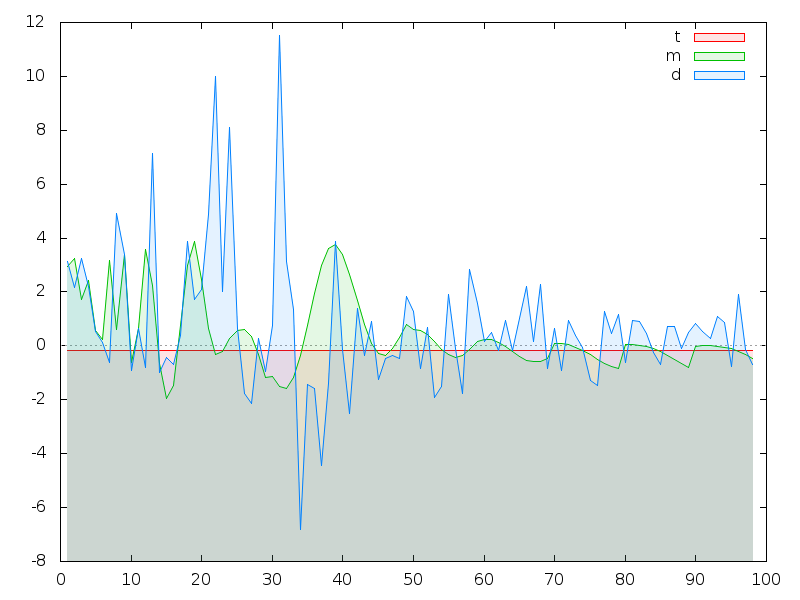
\includegraphics[width=\linewidth]{../wykresy/test4_int.png}
    \caption{Wykres całki dla testu 4 i $n=100$}
    \label{fig:test41}
  \end{minipage}
  \hspace{0.5cm}
  \begin{minipage}[b]{0.45\linewidth}
    \centering
    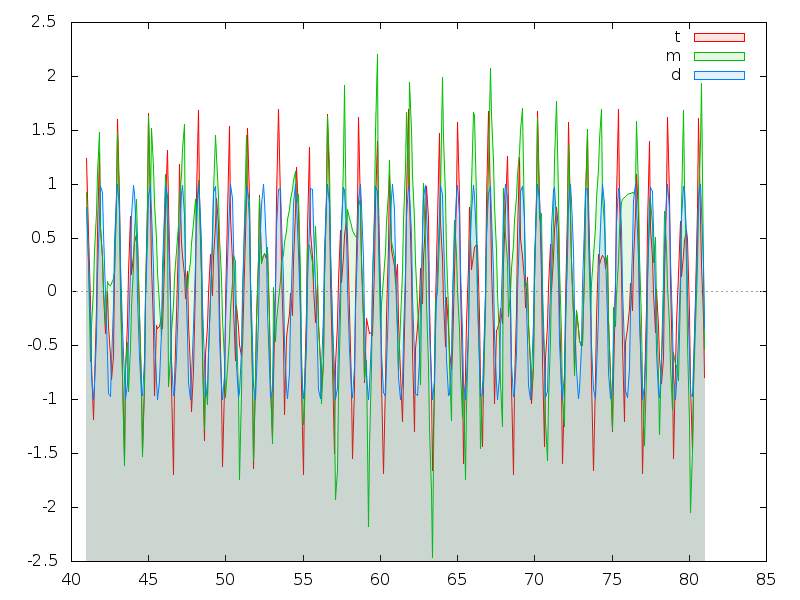
\includegraphics[width=\linewidth]{../wykresy/test4_spline.png}
    \caption{Wykres funkcji dla testu 4 i $n=100$}
    \label{fig:test42}
  \end{minipage}
\end{figure}
Powód tak kiepskich wyników jest dobrze widoczny: punkty kluczowe były zbyt rzadko położone, by oddać zachowanie funkcji tak szybko zmiennej.\\
{\small{\\Wykresy można znaleźć w katalogu "./wykresy". Dla każdego testu znajduje się tam wykres obrazujący zbieżność metody, dokładność przybliżenia funkcji przez NFSI3 oraz wykres całki. Z kolei numeryczne wartości są w plikach wymienionych przy opisie programu. }} 
\subsection{Wnioski}
Można z tego wnioskować, że omawiana metoda jest przydatna, jeśli szukamy szybkiego oszacowania całki z niedużą dokładnością - wystarczy wtedy wziąc $n$ dostateczne, by NFSI3 dość dobrze oddawało charakter funkcji, a następnie scałkować. Niestety jedyne oszacowanie błędu jest dane wzorem, który go dość grubo szacuje (poprzez maksimum czwartej pochodnej). Tak więc dla pewnych funkcji - takich, których normy jednostajne kolejnych pochodnych na danym przedziale nie są malejące - wymagałoby to dość dużego $n$.
\section{Zakończenie}
Z przeprowadzonych doświadczeń wynika, że metoda całkowania przez interpolacje NFSI3 jest lepsza od kwadratury Newtona-Cotesa, ponieważ jest zawsze zbieżna. Jednak czasem zbieżność ta pojawia się dopiero po przekroczeniu pewnej (dużej) liczby punktów kluczowych. Oprócz tego nie jest to szybka zbieżność. Wydaje się więc dobra dla szacowania wartości całki, a nie do precyzyjnego wyliczania jej wartości. Pozostaje rozstrzygnąć, czy do tych zastosowań nie jest lepsza np złożona metoda trapezów (ze wzorów wynikają bardzo podobne oszacowania błędu). Nie powinno tak być, ponieważ NFSI3 używa większej liczby parametrów (ma więcej danych o funkcji). Obie metody mają podobny koszt obliczeniowy. Pod względem zbieżności o wiele lepsza jednak jest metoda Romberga. Jest ona jednak kosztowniejsza od całkowania przez NFSI3, jednak ledwie pare iteracji (druga lub trzecia kolumna) powinny pozwolić osiągnąć poziom błędu taki, jak omawianej metody.
\end{document}

